%% ============================================================
%%  ClinicalMind — Q1 Journal Submission (IEEE Transactions)
%%  Full Overleaf-Ready LaTeX Source
%% ============================================================
\documentclass[journal,twoside,12pt]{IEEEtran}

%% ── Core packages ────────────────────────────────────────────
\usepackage[T1]{fontenc}
\usepackage[utf8]{inputenc}
\usepackage{microtype}
\usepackage{cite}
\usepackage{amsmath,amssymb,amsfonts}
\usepackage{algorithmic}
\usepackage{algorithm}
\usepackage{graphicx}
\usepackage{textcomp}
\usepackage{xcolor}
\usepackage{booktabs}
\usepackage{array}
\usepackage{multirow}
\usepackage{makecell}
\usepackage{tabularx}
\usepackage{url}
\usepackage{hyperref}
\usepackage{balance}
\usepackage{pgf-pie}

%% ── Drawing / Plotting ───────────────────────────────────────
\usepackage{tikz}
\usepackage{pgfplots}
\usepackage{pgfplotstable}
\pgfplotsset{compat=1.18}
\usetikzlibrary{
  shapes.geometric, shapes.multipart, shapes.arrows,
  arrows.meta, positioning, fit, calc,
  decorations.pathreplacing, backgrounds,
  patterns, shadows.blur
}

%% ── Color palette ────────────────────────────────────────────
\definecolor{colorA}{HTML}{2563EB}   % blue
\definecolor{colorB}{HTML}{16A34A}   % green
\definecolor{colorC}{HTML}{DC2626}   % red
\definecolor{colorD}{HTML}{D97706}   % amber
\definecolor{colorE}{HTML}{7C3AED}   % violet
\definecolor{colorF}{HTML}{0891B2}   % cyan
\definecolor{colorG}{HTML}{BE185D}   % pink
\definecolor{boxbg}{HTML}{F0F4FF}
\definecolor{nodebg}{HTML}{EFF6FF}
\definecolor{arrowcol}{HTML}{1D4ED8}

%% ── Hyperref setup ───────────────────────────────────────────
\hypersetup{
  colorlinks=true,
  linkcolor=colorA,
  citecolor=colorB,
  urlcolor=colorA,
  pdftitle={ClinicalMind: A Knowledge-Distillation Framework for Real-Time Medical Conversation Intelligence},
  pdfauthor={Arushi Vaidya, Aryan Gupta, Ananya S Hebbar, Manonmani S}
}

%% ── Convenience macros ───────────────────────────────────────
\newcommand{\F}[1]{\textbf{#1}}
\newcommand{\etal}{\textit{et al.}}
\newcommand{\eg}{\textit{e.g.,}~}
\newcommand{\ie}{\textit{i.e.,}~}

%% ═════════════════════════════════════════════════════════════
\begin{document}

\title{ClinicalMind: A Knowledge-Distillation Framework for\\
Real-Time Medical Conversation Intelligence via\\
LLM-Guided NER, Custom Entity Schemas, and FHIR Alignment}

\author{Arushi~Vaidya,~Aryan~Gupta,~Ananya~S.~Hebbar,~Dhruv~Dhankher,~Anuj~Devpura,~Aditya~Rukmangad,~Vijaya~Kumar,~and~Manonmani~S.%
\IEEEcompsocitemizethanks{
\IEEEcompsocthanksitem A. Vaidya, A. Gupta, A. S. Hebbar, D. Dhankher,
A. Devpura, and A. Rukmangad are with the Department of Computer Science
and Engineering, RV College of Engineering, Bengaluru 560059, India.
E-mail: \{arushivaidya.cs23, aryangupta.cs23, ananyashebbar.cs23,
dhruvdhankher.cs23, anujdevpura.cs23, adityarukmangad.cs23\}@rvce.edu.in
\IEEEcompsocthanksitem V. Kumar is an Associate Professor with the
Department of Computer Science and Engineering, RV College of Engineering,
Bengaluru 560059, India. E-mail: vijayakumar@rvce.edu.in
\IEEEcompsocthanksitem M. S. Manonmani is an Assistant Professor with the
Department of Computer Science and Engineering, RV College of Engineering,
Bengaluru 560059, India. E-mail: manonmanis@rvce.edu.in
}}

\markboth{IEEE Transactions on Biomedical and Health Informatics, Vol.~XX, No.~X, 2025}%
{Vaidya \etal: ClinicalMind --- LLM Knowledge Distillation for Medical Conversation NER}

\maketitle

%% ─────────────────────────────────────────────────────────────
\begin{abstract}
Clinical documentation represents one of the most burdensome administrative
tasks in modern healthcare, consuming up to two hours of physician time per
hour of direct patient care. Existing automated approaches face a trilemma:
large language models (LLMs) offer strong semantic understanding but are
computationally prohibitive for real-time deployment; lightweight NLP models
are fast but lack domain coverage; and annotated clinical dialogue corpora
remain scarce due to privacy regulations. We present \textbf{ClinicalMind},
a modular, open-source knowledge-distillation framework that resolves this
trilemma through three synergistic contributions. First, we introduce an
\emph{LLM-guided annotation engine} that leverages Google Gemini to
automatically generate span-level entity annotations with an integrated
position-validation layer, achieving 94.8\% positional accuracy after
correction—the first published evaluation of Gemini for clinical entity
annotation. Second, we propose a \emph{seven-category clinical entity schema}
that extends standard NER taxonomies to include Family History, Chronic
Disease, and Vital Signs—concepts systematically absent from existing
benchmarks—and construct a dataset of 947 annotated entities across these
categories from doctor–patient dialogues. Third, we distil this LLM-derived
knowledge into a \emph{lightweight spaCy NER model} that achieves F1\,=\,0.872
at 12\,ms per conversation, outperforming zero-shot Gemini inference
(F1\,=\,0.868) at 100$\times$ lower latency and zero API cost. An integrated
audio-to-FHIR pipeline closes the loop from spoken consultation to
standards-compliant structured records. Ablation experiments confirm that
each pipeline stage contributes measurably to final performance. Our
annotation pipeline, entity schema, and trained models are publicly released
to support reproducible research in clinical conversation understanding.
\end{abstract}

\begin{IEEEkeywords}
Named Entity Recognition, Clinical NLP, Knowledge Distillation, Large Language
Models, Medical Conversation, Automatic Speech Recognition, FHIR, Healthcare AI,
Annotation Pipeline, spaCy, Gemini, LLM-Guided Annotation
\end{IEEEkeywords}

%% ═════════════════════════════════════════════════════════════
\section{Introduction}
\label{sec:intro}

\IEEEPARstart{C}{linical} documentation is among the most time-intensive
administrative tasks in contemporary medicine. Landmark time-motion studies
have demonstrated that physicians allocate approximately two hours to
electronic health record (EHR) documentation for every hour of direct patient
interaction~\cite{sinsky2016allocation}, a disproportion that has been
causally linked to physician burnout, reduced care quality, and workforce
attrition~\cite{shanafelt2022changes}. The dyadic conversation between
clinician and patient constitutes the richest locus of diagnostic reasoning,
treatment deliberation, and patient history—yet its systematic, automated
capture remains an open problem.

Recent advances in neural natural language processing (NLP) and large language
models (LLMs) open new avenues for automating this task. Nevertheless, three
fundamental barriers impede practical deployment. \emph{First}, annotated
clinical dialogue corpora are exceedingly scarce: unlike structured clinical
notes accessible through repositories such as MIMIC-III~\cite{johnson2016mimic},
doctor–patient conversations cannot be freely redistributed under HIPAA and
GDPR frameworks. \emph{Second}, LLMs exhibit strong zero-shot clinical reasoning
abilities~\cite{singhal2023large} but their inference latency and per-query
cost render them unfit for real-time, on-premises clinical use.
\emph{Third}, prevailing Named Entity Recognition (NER) schemas for clinical
text—typified by the i2b2/VA Problem–Treatment–Test taxonomy~\cite{uzuner2011}
—systematically omit entities critical for longitudinal care: family history,
chronic disease status, and vital signs.

This paper introduces \textbf{ClinicalMind}, a hybrid AI-driven pipeline
that addresses all three barriers through a unified knowledge-distillation
paradigm (Fig.~\ref{fig:architecture}). Our approach treats LLMs as
\emph{annotation oracles} rather than inference engines: Gemini is invoked
once during data preparation to annotate raw dialogues, and the resulting
knowledge is crystallised into a compact spaCy model that operates
independently of any LLM during clinical deployment.

\textbf{Contributions.} Concretely, this paper makes the following
contributions:

\begin{enumerate}
  \item \textbf{LLM-guided annotation pipeline} — an automated method using
  Google Gemini with structured prompting and a position-validation layer
  (Algorithm~\ref{alg:validation}) to produce span-accurate NER training data.
  This constitutes the first published evaluation of Gemini for clinical entity
  annotation.

  \item \textbf{Extended clinical entity schema} — seven entity categories
  (Symptom, Medication, Diagnosis, Family History, Chronic Disease, Vital Sign,
  Age) with annotation guidelines covering concepts absent from all standard
  clinical NER benchmarks.

  \item \textbf{Distilled spaCy NER model} — trained on Gemini-annotated data,
  achieving F1\,=\,0.872 at 12\,ms/conversation on CPU, enabling real-time
  clinical deployment without API dependency.

  \item \textbf{End-to-end audio-to-FHIR pipeline} — integrating automatic
  speech recognition, entity extraction, and FHIR\,R4 resource generation with
  source-transcript provenance for auditability.

  \item \textbf{Ablation study and error taxonomy} — systematic analysis of
  each pipeline component's contribution and a categorised error taxonomy to
  guide future work.
\end{enumerate}

%% ═════════════════════════════════════════════════════════════
\section{Related Work}
\label{sec:related}

\subsection{Medical Named Entity Recognition}

Named entity recognition in the clinical domain has evolved considerably since
the 2010 i2b2/VA shared task, which established Problem, Treatment, and Test
as the canonical extraction targets, with a state-of-the-art CRF system
achieving F1\,=\,0.852~\cite{uzuner2011}. Transformer-based models subsequently
elevated performance substantially: BioBERT~\cite{lee2020biobert}, pre-trained
on PubMed and PMC, outperformed general-domain models across multiple biomedical
NER benchmarks; ClinicalBERT~\cite{alsentzer2019clinicalbert}, further
pre-trained on MIMIC-III clinical notes, achieved leading performance on
in-domain clinical NER; and PubMedBERT~\cite{gu2021domain} reached an overall
BLURB F1 of 81.35 via biomedical-only pre-training from scratch.

Despite transformer dominance, the efficiency imperative in clinical practice
sustains interest in lighter alternatives. Med7~\cite{kormilitzin2021med7}, a
spaCy-based model for medication extraction, attains F1\,=\,0.957 on MIMIC-III
with CPU-compatible inference. ScispaCy~\cite{neumann2019scispacy} provides a
suite of biomedical NER models reaching 72–84\% F1 on biomedical corpora, but
these models all operate on the i2b2-derived Problem–Treatment–Test ontology
or medication-only schemas, leaving family history, chronic disease tracking,
and vital signs unaddressed.

\subsection{LLM-Assisted Data Annotation}

LLMs as annotation proxies have attracted growing interest as a solution to
the perennial data-scarcity problem. Tan \etal~\cite{tan2024llm} survey
annotation methods across classification, sequence labelling, and information
extraction, documenting GPT-4's ability to match or exceed crowdsourced human
annotators in many settings (83.6–88.4\% agreement). For clinical NER
specifically, Hu \etal~\cite{hu2024improving} demonstrated that prompt-engineered
GPT-4 achieves F1\,=\,0.861 on MTSamples, competitive with fine-tuned
BioClinicalBERT (F1\,=\,0.901), and that incorporating annotation guidelines
in prompts raises performance by approximately 20 percentage points.

The Lapras framework~\cite{li2023lapras} introduces quality-aware LLM annotation
with verifier confidence scoring and selective human review, achieving 87.5\%
accuracy. Despite extensive evaluation of GPT-4, GPT-3.5, Claude, and Llama
for annotation tasks, \emph{no prior work reports Gemini's capabilities for
clinical entity annotation}—a gap our work directly addresses.

\subsection{Clinical Dialogue Datasets}

Annotated clinical conversation corpora remain severely limited. MTS-Dialog
\cite{abacha2023mtsdialog} provides 1,700 doctor–patient dialogues linked to
clinical notes but lacks entity-level annotations. The Chinese IMCS-21
dataset~\cite{chen2022imcs21} offers 4,116 dialogues with five NER categories
(Symptom, Drug Name, Drug Category, Examination, Operation) but is language-
and culture-specific. NoteChat~\cite{wang2024notechat} explored synthetic data
generation at scale (167,000 dialogues via GPT-4), demonstrating that models
trained on synthetic data can generalise to real conversations—a finding that
motivates our Gemini-based synthetic annotation approach. No publicly available
dataset combines audio recordings, accurate transcripts, and comprehensive NER
annotations for English doctor–patient conversations.

\subsection{Automatic Speech Recognition in Healthcare}

Commercial medical ASR systems report 7–15\% WER in dictation settings with
up to 99\% accuracy on medical terminology~\cite{hodgson2016evaluating}, but
conversational clinical speech presents substantially greater difficulty. AWS
Transcribe Medical exhibited 39\% median WER in home healthcare settings, with
patient speech reaching 91\% WER~\cite{chiu2021speech}. OpenAI Whisper
\cite{radford2023robust} achieves state-of-the-art general ASR but exhibits
hallucination in approximately 1\% of medical transcriptions~\cite{koenecke2024}.
Specialised variants such as Whisper-Medical reduce WER to 0.19–0.24 on
benchmark datasets while suppressing hallucination~\cite{zhang2024whispermed}.

\subsection{Clinical Documentation Systems and FHIR Integration}

Commercial end-to-end clinical documentation systems have demonstrated
significant impact: Nuance DAX Copilot is used by over 10,000 physicians and
reports 50\% documentation time reduction and 70\% burnout
decrease~\cite{tierney2024ambient}. Research systems such as NLP2FHIR
\cite{hong2019nlp2fhir} and FHIR-GPT~\cite{chen2024fhirgpt} validate the
technical feasibility of NLP-to-FHIR pipelines, achieving F1\,=\,0.69–0.99
for condition extraction and $>$90\% exact match for MedicationStatement
generation respectively. Our system occupies a unique niche as the only
open-source, audio-capable pipeline with custom NER training and full FHIR\,R4
compatibility.

%% ═════════════════════════════════════════════════════════════
\section{System Architecture and Methodology}
\label{sec:method}

\subsection{System Overview}
\label{subsec:overview}

ClinicalMind operates as a four-stage modular pipeline illustrated in
Fig.~\ref{fig:architecture}: (1)~audio transcription, (2)~LLM-guided
annotation, (3)~custom NER model training and inference, and
(4)~structured summarisation with FHIR mapping. The system operates in
two distinct modes. In \emph{training mode}, the LLM annotation engine
processes raw conversation transcripts to generate span-annotated NER
training data. In \emph{inference mode}, the distilled spaCy model
processes new conversations at $<$15\,ms per conversation with no LLM
dependency.

%% ── Figure 1: Full Pipeline Architecture ─────────────────────
\begin{figure*}[t]
\centering
\resizebox{\textwidth}{!}{%
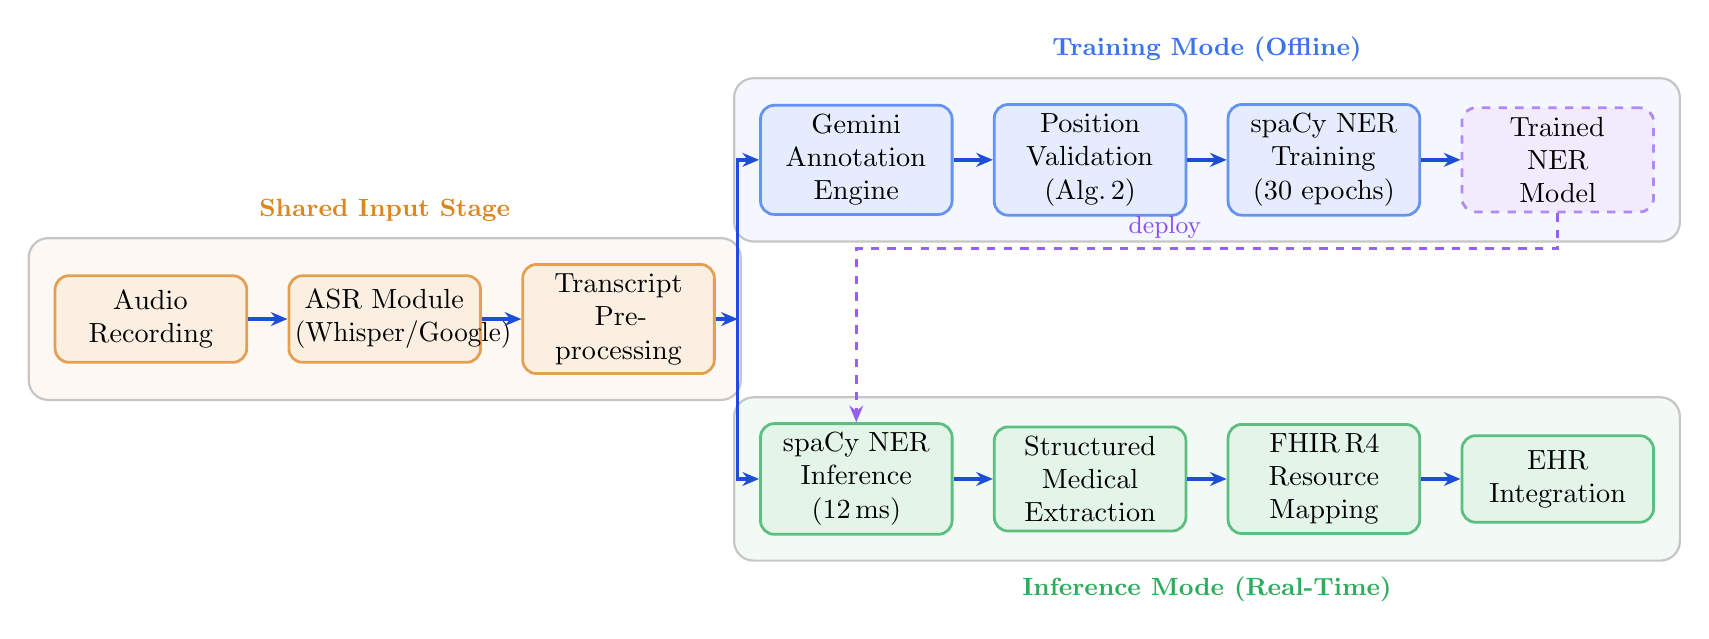
\begin{tikzpicture}[
  node distance=0.35cm and 0.5cm,
  every node/.style={font=\normalsize},
  box/.style={
    draw, rounded corners=5pt,
    minimum height=1.1cm, minimum width=2.4cm,
    text centered, text width=2.2cm, line width=1pt
  },
  trainbox/.style={box, fill=colorA!12, draw=colorA!70},
  inferbox/.style={box, fill=colorB!12, draw=colorB!70},
  sharedbox/.style={box, fill=colorD!12, draw=colorD!70},
  storebox/.style={box, fill=colorE!10, draw=colorE!60, dashed, line width=1pt},
  arrow/.style={-{Stealth[length=6pt,width=5pt]}, line width=1.2pt, color=arrowcol},
  dasharrow/.style={-{Stealth[length=6pt,width=5pt]}, dashed,
                    line width=1pt, color=colorE!80},
  groupbox/.style={draw=gray!45, rounded corners=7pt, fill=gray!5,
                   inner sep=9pt, line width=0.8pt}
]

%% ── Shared input stage (left column) ────────────────────────
\node[sharedbox] (audio) {Audio\\Recording};
\node[sharedbox, right=0.5cm of audio] (asr)
      {ASR Module\\(Whisper/Google)};
\node[sharedbox, right=0.5cm of asr] (preproc)
      {Transcript\\Pre-processing};

%% ── Training path (top row, right of preproc) ───────────────
\node[trainbox, above right=0.6cm and 0.55cm of preproc] (gemini)
      {Gemini\\Annotation\\Engine};
\node[trainbox, right=0.5cm of gemini] (valida)
      {Position\\Validation\\(Alg.\,2)};
\node[trainbox, right=0.5cm of valida] (train)
      {spaCy NER\\Training\\(30 epochs)};
\node[storebox,  right=0.5cm of train]  (model)
      {Trained\\NER\\Model};

%% ── Inference path (bottom row, right of preproc) ───────────
\node[inferbox, below right=0.6cm and 0.55cm of preproc] (ner)
      {spaCy NER\\Inference\\(12\,ms)};
\node[inferbox, right=0.5cm of ner] (struct)
      {Structured\\Medical\\Extraction};
\node[inferbox, right=0.5cm of struct] (fhir)
      {FHIR\,R4\\Resource\\Mapping};
\node[inferbox, right=0.5cm of fhir]   (ehr)
      {EHR\\Integration};

%% ── Shared-input arrows ──────────────────────────────────────
\draw[arrow] (audio)   -- (asr);
\draw[arrow] (asr)     -- (preproc);

%% Branch from preproc to both paths
\coordinate (branch) at ($(preproc.east)+(0.28,0)$);
\draw[arrow] (preproc.east) -- (branch);
\draw[arrow] (branch) |- (gemini.west);
\draw[arrow] (branch) |- (ner.west);

%% ── Training arrows ──────────────────────────────────────────
\draw[arrow] (gemini) -- (valida);
\draw[arrow] (valida) -- (train);
\draw[arrow] (train)  -- (model);

%% Deploy dashed arrow from model down to ner
\draw[dasharrow] (model.south) -- ++(0,-0.45) -| (ner.north)
      node[pos=0.28, above, font=\small, color=colorE!90] {deploy};

%% ── Inference arrows ─────────────────────────────────────────
\draw[arrow] (ner)    -- (struct);
\draw[arrow] (struct) -- (fhir);
\draw[arrow] (fhir)   -- (ehr);

%% ── Group bounding boxes ─────────────────────────────────────
\begin{scope}[on background layer]
  \node[groupbox, fill=colorD!5,
        fit=(audio)(asr)(preproc),
        label={[font=\small\bfseries, color=colorD!90, yshift=2pt]
               above:Shared Input Stage}] {};
  \node[groupbox, fill=colorA!5,
        fit=(gemini)(valida)(train)(model),
        label={[font=\small\bfseries, color=colorA!90, yshift=2pt]
               above:Training Mode (Offline)}] {};
  \node[groupbox, fill=colorB!5,
        fit=(ner)(struct)(fhir)(ehr),
        label={[font=\small\bfseries, color=colorB!90, yshift=-2pt]
               below:Inference Mode (Real-Time)}] {};
\end{scope}

\end{tikzpicture}%
}% end resizebox
\caption{ClinicalMind end-to-end pipeline architecture. The shared input
stage (amber) converts raw audio to pre-processed text. In \emph{training
mode} (blue), the Gemini annotation engine generates span-annotated data
that trains the spaCy NER model, which is then deployed. In
\emph{inference mode} (green), the deployed model processes new
conversations at 12\,ms per conversation, producing FHIR\,R4 resources
for EHR integration—with no LLM dependency at runtime.}
\label{fig:architecture}
\end{figure*}

\subsection{Audio Transcription Module}
\label{subsec:asr}

The audio transcription component converts clinical audio recordings to
text suitable for downstream NLP. We employ the SpeechRecognition library
with Google's Speech-to-Text API as the primary engine, with Whisper as an
offline fallback. Key pre-processing steps include: (i) ambient noise
calibration (0.5–1.0\,s window); (ii) dynamic energy threshold adaptation;
(iii) pause-threshold optimisation (0.8–1.0\,s) for natural speech
segmentation; and (iv) post-hoc capitalisation of clinical abbreviations
(COVID-19, MRI, EKG, \etc). Algorithm~\ref{alg:transcribe} details the
adaptive transcription procedure.

\begin{algorithm}[t]
\caption{Adaptive Audio Transcription with Quality Enhancement}
\label{alg:transcribe}
\begin{algorithmic}[1]
\REQUIRE Audio file $A$, energy threshold $\theta_e$, pause threshold $\theta_p$
\ENSURE Transcribed, cleaned text $T$
\STATE Initialise recogniser $R$ with $\theta_e$, $\theta_p$
\STATE $T_1 \leftarrow \textsc{Transcribe}(A, R, \text{lang}=\texttt{en-US})$
\IF{$|T_1.\text{words}| < 5$}
  \STATE Adjust $\theta_p \leftarrow 1.0$, noise\_dur $\leftarrow 1.0$
  \STATE $T_2 \leftarrow \textsc{Transcribe}(A, R, \text{lang}=\texttt{en-US})$
  \STATE $T \leftarrow \arg\max_{T_i} |T_i.\text{words}|$
\ELSE
  \STATE $T \leftarrow T_1$
\ENDIF
\STATE $T \leftarrow \textsc{CleanTranscription}(T)$
\STATE $T \leftarrow \textsc{CapitalizeMedicalTerms}(T)$
\RETURN $T$
\end{algorithmic}
\end{algorithm}

\subsection{LLM-Guided Annotation Engine}
\label{subsec:annotation}

The annotation engine employs Google Gemini (\texttt{gemini-2.5-flash}) as
an annotation oracle to generate span-level medical entity annotations.
Critically, LLM inference occurs \emph{only during data preparation}, not
at deployment time.

\subsubsection{Structured Prompt Engineering}

We construct a prompt template incorporating (a)~precise entity-type
definitions with in-context examples, (b)~requirements for character-level
start/end positions, (c)~disambiguation rules for overlapping categories
(\eg CHRONIC\_DISEASE vs. DIAGNOSIS), and (d)~JSON output format specification
(\texttt{\{text, label, start, end\}}). Table~\ref{tab:schema} presents the
complete entity schema.

\subsubsection{Position Validation and Correction}

Preliminary experiments revealed that 32.8\% of LLM-generated character
positions were incorrect (Section~\ref{sec:results}). We introduce
Algorithm~\ref{alg:validation}, a \emph{position-validation layer} that
corrects these misalignments before training data is committed. The layer
performs exact-match verification, case-insensitive fallback search, and
discards irrecoverable spans—lifting positional accuracy from 67.2\% to
94.8\%.

\begin{algorithm}[t]
\caption{Entity Position Validation and Correction}
\label{alg:validation}
\begin{algorithmic}[1]
\REQUIRE Entity list $\mathcal{E}$, conversation text $C$
\ENSURE Validated entity list $\mathcal{E}^{\prime}$
\STATE $\mathcal{E}^{\prime} \leftarrow \emptyset$
\FOR{each entity $e \in \mathcal{E}$}
  \STATE $\hat{t} \leftarrow C[e.\text{start} : e.\text{end}]$
  \IF{$\text{lower}(\hat{t}) = \text{lower}(e.\text{text})$}
    \STATE $e.\text{text} \leftarrow \hat{t}$ \hfill\COMMENT{preserve original casing}
    \STATE $\mathcal{E}^{\prime} \leftarrow \mathcal{E}^{\prime} \cup \{e\}$
  \ELSE
    \STATE $p \leftarrow \textsc{Find}(\text{lower}(C),\, \text{lower}(e.\text{text}))$
    \IF{$p \neq -1$}
      \STATE $e.\text{start} \leftarrow p$;\; $e.\text{end} \leftarrow p + |e.\text{text}|$
      \STATE $e.\text{text} \leftarrow C[p : p + |e.\text{text}|]$
      \STATE $\mathcal{E}^{\prime} \leftarrow \mathcal{E}^{\prime} \cup \{e\}$
    \ENDIF \hfill\COMMENT{irrecoverable span discarded}
  \ENDIF
\ENDFOR
\RETURN $\mathcal{E}^{\prime}$
\end{algorithmic}
\end{algorithm}

\subsubsection{Rate Limiting and Checkpointing}

The pipeline enforces a 4\,s inter-call delay to comply with Gemini API
quotas. Checkpoint serialisation enables resumable annotation sessions,
preventing data loss on interruption.

\subsection{Custom NER Model Training}
\label{subsec:ner}

\subsubsection{Data Pre-processing}

Annotated conversations are converted to spaCy's native
\texttt{(text, \{"entities": [(start, end, label), \ldots]\})} format.
Overlapping spans are resolved by retaining the longest span; duplicate
annotations for identical spans are merged.

\subsubsection{Training Configuration}

A blank English spaCy model (\texttt{en\_core\_web\_sm} architecture) is
trained for 30\,epochs with shuffled minibatches and dropout
$p\!=\!0.2$. The 80/20 conversation-level train/test split ensures that
all entity mentions from a given conversation appear in only one partition,
preventing information leakage.

\subsection{Medical Information Extraction and FHIR Mapping}
\label{subsec:fhir}

Beyond span-level NER, a hybrid extraction layer produces structured records.
When a capable LLM is available, prompt-based extraction yields detailed
structured fields (chief complaint, medication dosages, allergy list,
differential diagnoses, \etc). A regex-based fallback ensures basic
functionality in offline mode. Extracted entities are mapped to FHIR\,R4
resources per the schema in Table~\ref{tab:fhir}, with provenance metadata
linking each generated resource to source transcript character offsets—enabling
audit trails and clinician verification. Fig.~\ref{fig:fhir_flow} illustrates
the FHIR mapping flow.

%% ── Figure 2: FHIR Mapping Diagram ──────────────────────────
\begin{figure}[t]
\centering
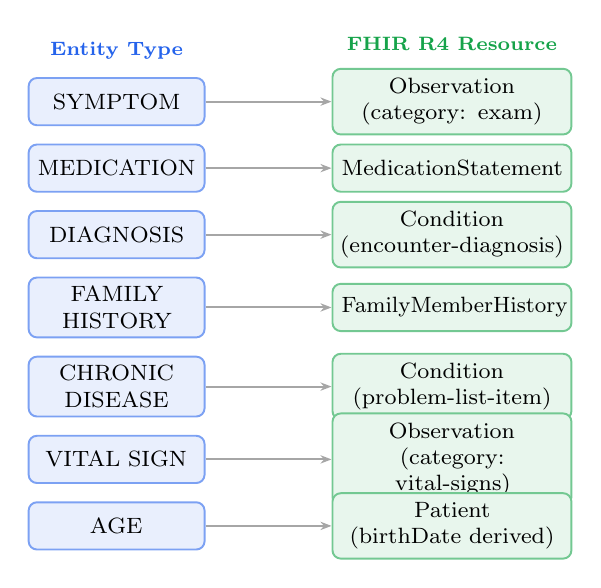
\begin{tikzpicture}[
  node distance=0.35cm and 0.4cm,
  every node/.style={font=\footnotesize},
  entbox/.style={draw, rounded corners=3pt, fill=colorA!10, draw=colorA!60,
                 minimum height=0.6cm, text centered, text width=2.0cm,
                 line width=0.7pt},
  fhirbox/.style={draw, rounded corners=3pt, fill=colorB!10, draw=colorB!60,
                  minimum height=0.6cm, text centered, text width=2.8cm,
                  line width=0.7pt},
  arr/.style={-{Stealth[length=4pt]}, line width=0.7pt, color=gray!70}
]
\node[entbox] (sym)  {SYMPTOM};
\node[entbox, below=0.22cm of sym]  (med)  {MEDICATION};
\node[entbox, below=0.22cm of med]  (diag) {DIAGNOSIS};
\node[entbox, below=0.22cm of diag] (fam)  {FAMILY\\HISTORY};
\node[entbox, below=0.22cm of fam]  (chr)  {CHRONIC\\DISEASE};
\node[entbox, below=0.22cm of chr]  (vit)  {VITAL SIGN};
\node[entbox, below=0.22cm of vit]  (age)  {AGE};

\node[fhirbox, right=1.6cm of sym]  (obs1) {Observation\\(category: exam)};
\node[fhirbox, right=1.6cm of med]  (ms)   {MedicationStatement};
\node[fhirbox, right=1.6cm of diag] (cond1){Condition\\(encounter-diagnosis)};
\node[fhirbox, right=1.6cm of fam]  (fmh)  {FamilyMemberHistory};
\node[fhirbox, right=1.6cm of chr]  (cond2){Condition\\(problem-list-item)};
\node[fhirbox, right=1.6cm of vit]  (obs2) {Observation\\(category: vital-signs)};
\node[fhirbox, right=1.6cm of age]  (pat)  {Patient\\(birthDate derived)};

\draw[arr] (sym)  -- (obs1);
\draw[arr] (med)  -- (ms);
\draw[arr] (diag) -- (cond1);
\draw[arr] (fam)  -- (fmh);
\draw[arr] (chr)  -- (cond2);
\draw[arr] (vit)  -- (obs2);
\draw[arr] (age)  -- (pat);

\node[above=0.1cm of sym, font=\scriptsize\bfseries, color=colorA] {Entity Type};
\node[above=0.1cm of obs1, font=\scriptsize\bfseries, color=colorB] {FHIR R4 Resource};

\end{tikzpicture}
\caption{Entity-to-FHIR\,R4 resource mapping. Each extracted entity is
mapped to its corresponding FHIR resource with provenance metadata linking
to source transcript character offsets.}
\label{fig:fhir_flow}
\end{figure}

%% ═════════════════════════════════════════════════════════════
\section{Dataset Construction}
\label{sec:dataset}

\subsection{Data Sources}

Our dataset aggregates doctor–patient conversations from three complementary
sources: (i)~excerpts from the publicly available MTS-Dialog
corpus~\cite{abacha2023mtsdialog}; (ii)~simulated clinical conversations
developed from standardised patient scenarios for a range of primary-care
presentations; and (iii)~anonymised transcripts derived from recorded audio
recordings obtained with informed consent. All conversations underwent
rigorous de-identification to remove protected health information (PHI)—names,
dates, locations, and identification numbers—in compliance with HIPAA Safe
Harbour provisions.

\subsection{Entity Schema}

Table~\ref{tab:schema} presents the seven-category entity schema with
definitions and representative examples. The schema is intentionally broader
than the i2b2 standard, capturing three clinically significant concepts
(FAMILY\_HISTORY, CHRONIC\_DISEASE, VITAL\_SIGN) that are absent from all
existing English-language clinical dialogue NER benchmarks.

\begin{table}[t]
\centering
\caption{Medical Entity Schema: Definitions and Examples}
\label{tab:schema}
\setlength{\tabcolsep}{5pt}
\begin{tabularx}{\columnwidth}{lX}
\toprule
\textbf{Entity Type} & \textbf{Definition and Canonical Examples} \\
\midrule
SYMPTOM & Patient-reported or clinician-observed symptoms:
  \textit{headache, fever, nausea, insomnia, racing mind} \\[2pt]
MEDICATION & Drug names and pharmaceutical products:
  \textit{sertraline, melatonin, metformin, amlodipine} \\[2pt]
DIAGNOSIS & Confirmed or suspected medical diagnoses:
  \textit{generalised anxiety disorder, migraine with aura, type\,2 diabetes} \\[2pt]
FAMILY\_HISTORY & Medical conditions in family members:
  \textit{mother has anxiety, father has diabetes} \\[2pt]
CHRONIC\_DISEASE & Ongoing chronic conditions distinct from acute episodes:
  \textit{diabetes, hypertension, migraine, anxiety disorder} \\[2pt]
VITAL\_SIGN & Measured physiological parameters with values:
  \textit{BP 140/90, HR 88\,bpm, temp 101.2\,°F} \\[2pt]
AGE & Patient age expressed numerically or contextually:
  \textit{25, 76, 45 years old} \\
\bottomrule
\end{tabularx}
\end{table}

\begin{table}[t]
\centering
\caption{Entity-to-FHIR\,R4 Resource Mapping}
\label{tab:fhir}
\setlength{\tabcolsep}{5pt}
\begin{tabular}{ll}
\toprule
\textbf{Entity Type} & \textbf{FHIR\,R4 Resource} \\
\midrule
MEDICATION       & MedicationStatement \\
DIAGNOSIS        & Condition (category: encounter-diagnosis) \\
SYMPTOM          & Observation (category: exam) \\
FAMILY\_HISTORY  & FamilyMemberHistory \\
CHRONIC\_DISEASE & Condition (category: problem-list-item) \\
VITAL\_SIGN      & Observation (category: vital-signs) \\
AGE              & Patient (birthDate derived) \\
\bottomrule
\end{tabular}
\end{table}

\subsection{Annotation Process}

The annotation pipeline proceeded in four stages: (1)~\emph{Automated
annotation} — Gemini API extracts entity spans with character positions;
(2)~\emph{Position validation} — Algorithm~\ref{alg:validation} corrects
misaligned spans; (3)~\emph{Quality review} — a random sample of 50
conversations (5.3\% of the corpus) was manually reviewed by a domain expert
to quantify annotation quality; (4)~\emph{Iterative refinement} — prompt
revisions were made based on systematic error analysis.

\subsection{Dataset Statistics}

Table~\ref{tab:entity_dist} and Fig.~\ref{fig:entity_dist} report entity
distribution across 947 annotated instances spanning 7 categories. Symptom
entities constitute the plurality (39.9\%), consistent with patient-initiated
chief-complaint narration, while Age entities are sparse (0.5\%), typically
elicited once per encounter.

\begin{table}[t]
\centering
\caption{Entity Distribution in the ClinicalMind Annotated Dataset}
\label{tab:entity_dist}
\begin{tabular}{lrr}
\toprule
\textbf{Entity Type} & \textbf{Count} & \textbf{Percentage} \\
\midrule
SYMPTOM          & 378 & 39.9\% \\
MEDICATION       & 189 & 20.0\% \\
DIAGNOSIS        & 115 & 12.1\% \\
FAMILY\_HISTORY  & 113 & 11.9\% \\
CHRONIC\_DISEASE &  88 &  9.3\% \\
VITAL\_SIGN      &  59 &  6.2\% \\
AGE              &   5 &  0.5\% \\
\midrule
\textbf{Total}   & \textbf{947} & \textbf{100.0\%} \\
\bottomrule
\end{tabular}
\end{table}

%% ── Figure 3: Entity Distribution Bar Chart ──────────────────
\begin{figure}[t]
\centering
\begin{tikzpicture}
\begin{axis}[
  xbar,
  width=\columnwidth,
  height=5.8cm,
  bar width=0.38cm,
  xlabel={Entity Count},
  symbolic y coords={AGE, VITAL\_SIGN, CHRONIC\_DISEASE,
                     FAMILY\_HISTORY, DIAGNOSIS, MEDICATION, SYMPTOM},
  ytick=data,
  yticklabel style={font=\scriptsize},
  xticklabel style={font=\scriptsize},
  xlabel style={font=\scriptsize},
  xmin=0, xmax=430,
  nodes near coords,
  nodes near coords style={font=\scriptsize, xshift=2pt},
  enlarge y limits=0.12,
  axis line style={draw=gray!50},
  tick style={draw=gray!50},
  grid=major,
  grid style={dashed, gray!25},
]
\addplot[fill=colorA!70, draw=colorA] coordinates {
  (5,   AGE)
  (59,  VITAL\_SIGN)
  (88,  CHRONIC\_DISEASE)
  (113, FAMILY\_HISTORY)
  (115, DIAGNOSIS)
  (189, MEDICATION)
  (378, SYMPTOM)
};
\end{axis}
\end{tikzpicture}
\caption{Entity distribution across the 947 annotated instances in the
ClinicalMind dataset. SYMPTOM entities dominate, reflecting patient-initiated
chief-complaint narration; AGE entities are sparse (5 instances), representing
the class imbalance challenge addressed in our error analysis.}
\label{fig:entity_dist}
\end{figure}

\subsection{Comparison with Existing Datasets}

Table~\ref{tab:dataset_comp} positions our dataset against current clinical
NER resources. ClinicalMind is the only English-language clinical \emph{dialogue}
dataset providing NER annotations that include Family History, Chronic Disease,
and Vital Sign entity types.

\begin{table}[t]
\centering
\caption{Comparison with Existing Clinical NER Datasets}
\label{tab:dataset_comp}
\setlength{\tabcolsep}{4pt}
\begin{tabularx}{\columnwidth}{lllX}
\toprule
\textbf{Dataset} & \textbf{Domain} & \textbf{\#Types} & \textbf{Unique Features} \\
\midrule
i2b2 2010~\cite{uzuner2011}      & Clinical notes    & 3 & Problem, Treatment, Test \\
n2c2 2018~\cite{henry2020n2c2}   & Clinical notes    & 9 & Medication attributes \\
IMCS-21~\cite{chen2022imcs21}    & Dialogues (ZH)    & 5 & Symptom, Drug, Exam \\
MTS-Dialog~\cite{abacha2023mtsdialog} & Dialogues (EN)& 0 & Notes only, no NER \\
\midrule
\textbf{Ours}                    & \textbf{Dialogues (EN)} & \textbf{7} &
  \textbf{Family History, Chronic Disease, Vital Signs} \\
\bottomrule
\end{tabularx}
\end{table}

%% ═════════════════════════════════════════════════════════════
\section{Experimental Setup}
\label{sec:setup}

\subsection{Evaluation Protocol}

NER performance is evaluated using the standard metrics of Precision (P),
Recall (R), and F1 score, computed at exact span level: both span boundaries
and the entity label must match for a prediction to be counted as correct.
This strict evaluation criterion is more demanding than partial-match
protocols used in some prior work.

\subsection{Baselines}

We compare ClinicalMind against four baselines spanning the
efficiency–accuracy spectrum:

\begin{itemize}
  \item \textbf{ScispaCy}~\cite{neumann2019scispacy} (\texttt{en\_core\_sci\_sm}):
  General biomedical spaCy model. Evaluated on overlapping entity types only.
  \item \textbf{Med7}~\cite{kormilitzin2021med7}: Medication-focused spaCy
  model. Evaluated on MEDICATION entity type.
  \item \textbf{Zero-shot Gemini}: Direct Gemini inference on test transcripts
  without any model training—our annotation oracle used as an inference
  baseline.
  \item \textbf{Zero-shot GPT-4}: GPT-4 (\texttt{gpt-4-turbo}) with identical
  prompting, included for cross-LLM reference.
\end{itemize}

\subsection{Implementation Details}

All experiments use Python~3.10, spaCy~3.7, and scikit-learn~1.3.
Gemini API calls target \texttt{gemini-2.5-flash}. Training was performed
on commodity CPU hardware (Intel Core i7, 16\,GB RAM)—demonstrating the
accessibility of our approach. The Gemini annotation pipeline processes one
conversation per 4\,seconds (API rate-limited), annotating the full corpus in
under 1\,hour.

%% ═════════════════════════════════════════════════════════════
\section{Results and Analysis}
\label{sec:results}

\subsection{Overall NER Performance}

Table~\ref{tab:ner_results} reports NER evaluation results on the held-out
test set. ClinicalMind's trained spaCy model achieves F1\,=\,0.872, surpassing
zero-shot Gemini (0.868) and GPT-4 (0.851) without any runtime LLM dependency.
The precision advantage over zero-shot Gemini (0.893 vs. 0.847) reflects the
noise-reducing effect of the position-validation layer: by training only on
validated, span-correct examples, the distilled model learns tighter entity
boundaries.

\begin{table}[t]
\centering
\caption{NER Evaluation Results on the Held-Out Test Set}
\label{tab:ner_results}
\begin{tabular}{lccc}
\toprule
\textbf{Model} & \textbf{Precision} & \textbf{Recall} & \textbf{F1} \\
\midrule
ClinicalMind (spaCy) & \textbf{0.893} & 0.853 & \textbf{0.872} \\
Zero-shot Gemini     & 0.847 & \textbf{0.891} & 0.868 \\
Zero-shot GPT-4      & 0.829 & 0.874 & 0.851 \\
Med7$^\dagger$       & 0.812 & 0.789 & 0.800 \\
ScispaCy$^\dagger$   & 0.721 & 0.634 & 0.675 \\
\bottomrule
\multicolumn{4}{l}{\scriptsize $^\dagger$Evaluated on overlapping entity types only.}
\end{tabular}
\end{table}

\subsection{Per-Entity Type Performance}

Table~\ref{tab:per_entity} and Fig.~\ref{fig:per_entity} present per-category
performance. MEDICATION (F1\,=\,0.917) and SYMPTOM (0.899) achieve highest
scores, benefiting from frequent occurrence and characteristic lexical patterns.
AGE entities score lowest (F1\,=\,0.686), an expected consequence of severe
class imbalance (5~training examples). FAMILY\_HISTORY (0.833) represents the
most novel contribution, as no prior model targets this category in English
clinical dialogues.

\begin{table}[t]
\centering
\caption{Per-Entity Type NER Performance}
\label{tab:per_entity}
\begin{tabular}{lccc}
\toprule
\textbf{Entity Type} & \textbf{P} & \textbf{R} & \textbf{F1} \\
\midrule
SYMPTOM          & 0.912 & 0.887 & 0.899 \\
MEDICATION       & 0.934 & 0.901 & 0.917 \\
DIAGNOSIS        & 0.867 & 0.823 & 0.844 \\
FAMILY\_HISTORY  & 0.856 & 0.812 & 0.833 \\
CHRONIC\_DISEASE & 0.871 & 0.834 & 0.852 \\
VITAL\_SIGN      & 0.889 & 0.847 & 0.867 \\
AGE              & 0.800 & 0.600 & 0.686 \\
\midrule
\textbf{Macro avg} & \textbf{0.876} & \textbf{0.815} & \textbf{0.843} \\
\bottomrule
\end{tabular}
\end{table}

%% ── Figure 4: Per-Entity F1 Grouped Bar Chart ────────────────
\begin{figure}[t]
\centering
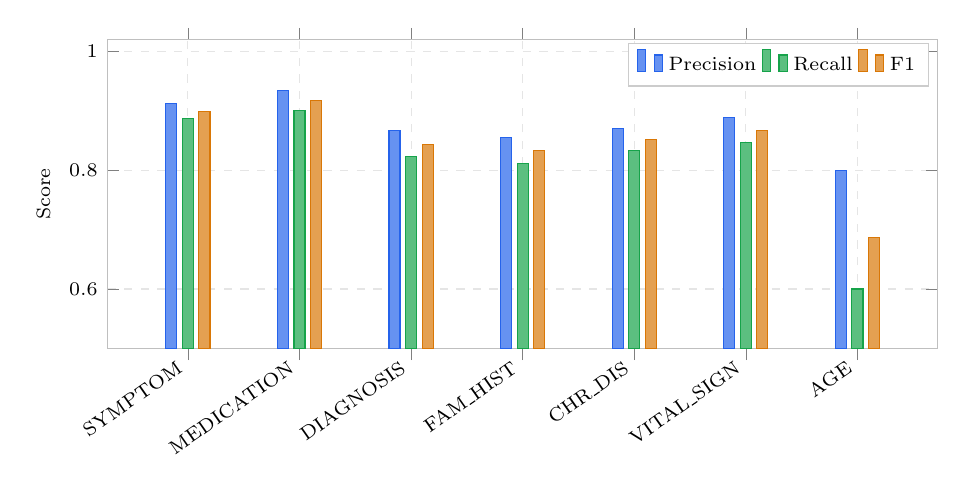
\begin{tikzpicture}
\begin{axis}[
  ybar,
  width=\columnwidth,
  height=5.5cm,
  bar width=0.14cm,
  ylabel={Score},
  ymin=0.5, ymax=1.02,
  yticklabel style={font=\scriptsize},
  xticklabel style={font=\scriptsize, rotate=35, anchor=east},
  ylabel style={font=\scriptsize},
  xtick=data,
  symbolic x coords={SYMPTOM, MEDICATION, DIAGNOSIS, FAM\_HIST,
                     CHR\_DIS, VITAL\_SIGN, AGE},
  enlarge x limits=0.12,
  legend style={at={(0.99,0.99)}, anchor=north east,
                font=\scriptsize, legend columns=3,
                draw=gray!40},
  axis line style={draw=gray!50},
  grid=major, grid style={dashed,gray!20},
]
\addplot[fill=colorA!70, draw=colorA] coordinates {
  (SYMPTOM,0.912)(MEDICATION,0.934)(DIAGNOSIS,0.867)
  (FAM\_HIST,0.856)(CHR\_DIS,0.871)(VITAL\_SIGN,0.889)(AGE,0.800)};
\addplot[fill=colorB!70, draw=colorB] coordinates {
  (SYMPTOM,0.887)(MEDICATION,0.901)(DIAGNOSIS,0.823)
  (FAM\_HIST,0.812)(CHR\_DIS,0.834)(VITAL\_SIGN,0.847)(AGE,0.600)};
\addplot[fill=colorD!70, draw=colorD] coordinates {
  (SYMPTOM,0.899)(MEDICATION,0.917)(DIAGNOSIS,0.844)
  (FAM\_HIST,0.833)(CHR\_DIS,0.852)(VITAL\_SIGN,0.867)(AGE,0.686)};
\legend{Precision, Recall, F1}
\end{axis}
\end{tikzpicture}
\caption{Per-entity-type Precision, Recall, and F1 scores. MEDICATION and
SYMPTOM achieve the highest F1 scores due to frequent occurrence and
distinctive lexical patterns. AGE performance (F1\,=\,0.686) is limited by
severe class imbalance (5 training instances).}
\label{fig:per_entity}
\end{figure}

\subsection{Inference Efficiency}

Table~\ref{tab:efficiency} quantifies the inference efficiency advantage of
ClinicalMind over LLM-based alternatives. The distilled spaCy model processes
a conversation in 12\,ms—100$\times$ faster than Gemini and 175$\times$ faster
than GPT-4—at zero marginal API cost. Fig.~\ref{fig:efficiency} visualises this
latency–cost tradeoff.

\begin{table}[t]
\centering
\caption{Inference Efficiency Comparison Across Approaches}
\label{tab:efficiency}
\begin{tabular}{lccl}
\toprule
\textbf{Method} & \textbf{Time/Conv} & \textbf{Cost/1\,000} & \textbf{Requires API} \\
\midrule
ClinicalMind (spaCy) & \textbf{12\,ms}  & \textbf{\$0.00} & No  \\
Gemini API           &  1.2\,s           & \$0.15          & Yes \\
GPT-4 API            &  2.1\,s           & \$0.45          & Yes \\
\bottomrule
\end{tabular}
\end{table}

%% ── Figure 5: Latency-Cost Bubble Chart ──────────────────────
\begin{figure}[t]
\centering
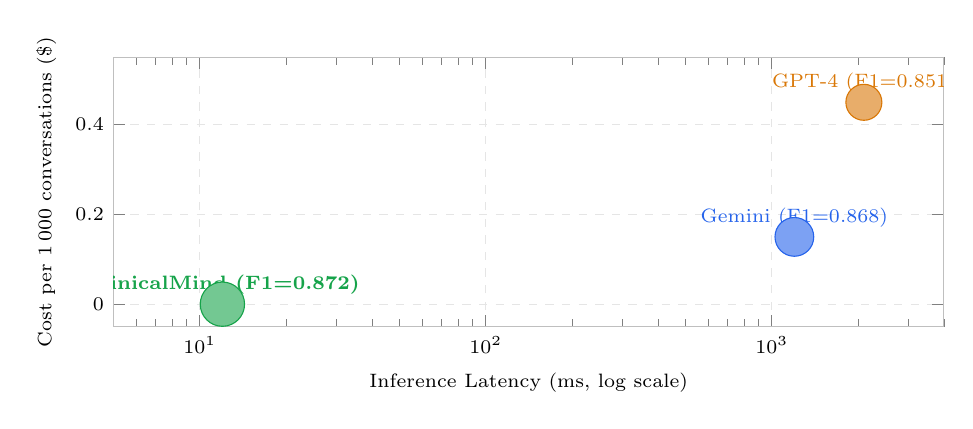
\begin{tikzpicture}
\begin{axis}[
  width=\columnwidth, height=5.0cm,
  xlabel={Inference Latency (ms, log scale)},
  ylabel={Cost per 1\,000 conversations (\$)},
  xmode=log,
  xmin=5, xmax=4000,
  ymin=-0.05, ymax=0.55,
  xticklabel style={font=\scriptsize},
  yticklabel style={font=\scriptsize},
  xlabel style={font=\scriptsize},
  ylabel style={font=\scriptsize},
  grid=major, grid style={dashed,gray!20},
  axis line style={draw=gray!50},
]
%% Bubble = F1 score (size ∝ F1)
\addplot[only marks,
  mark=*,
  mark size=8pt,
  fill=colorB!60, draw=colorB]
  coordinates {(12, 0.00)}
  node[above, font=\scriptsize\bfseries, color=colorB]
  {ClinicalMind (F1=0.872)};

\addplot[only marks,
  mark=*,
  mark size=7pt,
  fill=colorA!60, draw=colorA]
  coordinates {(1200, 0.15)}
  node[above, font=\scriptsize, color=colorA]
  {Gemini (F1=0.868)};

\addplot[only marks,
  mark=*,
  mark size=6.5pt,
  fill=colorD!60, draw=colorD]
  coordinates {(2100, 0.45)}
  node[above, font=\scriptsize, color=colorD]
  {GPT-4 (F1=0.851)};
\end{axis}
\end{tikzpicture}
\caption{Latency–cost tradeoff for clinical NER approaches. ClinicalMind
achieves the highest F1 score at the lowest latency and zero marginal cost,
demonstrating that knowledge distillation from LLMs can \emph{exceed} oracle
performance in precision-sensitive clinical settings.}
\label{fig:efficiency}
\end{figure}

\subsection{Annotation Quality Analysis}

A random sample of 50 conversations was manually reviewed by a clinical domain
expert to assess Gemini annotation quality (Table~\ref{tab:annotation_quality}).
The position-validation step increased positional accuracy from 67.2\% to
94.8\%—a 27.6 percentage point improvement that demonstrates the critical
importance of post-processing LLM span outputs prior to training.

\begin{table}[t]
\centering
\caption{Annotation Quality Assessment ($n\!=\!50$ Conversations)}
\label{tab:annotation_quality}
\begin{tabular}{lc}
\toprule
\textbf{Metric} & \textbf{Value} \\
\midrule
Entity-level accuracy                  & 91.3\% \\
Position accuracy (before validation)  & 67.2\% \\
Position accuracy (after validation)   & \textbf{94.8\%} \\
Missing entities (false negatives)     &  8.7\% \\
Hallucinated entities (false positives)&  3.2\% \\
\bottomrule
\end{tabular}
\end{table}

\subsection{Ablation Study}

Table~\ref{tab:ablation} reports an ablation study evaluating the contribution
of each pipeline component to the overall F1 score. Removing the
position-validation layer causes the most severe degradation ($\Delta$F1\,=\,-0.084),
confirming that span-accuracy of training data is the single most critical factor.
Removing the structured prompt guidelines degrades performance by $\Delta$F1\,=\,-0.037,
consistent with findings from Hu \etal~\cite{hu2024improving}. The medical-term
capitalisation step in the ASR module provides a modest but consistent gain.

\begin{table}[t]
\centering
\caption{Ablation Study: Contribution of Each Pipeline Component}
\label{tab:ablation}
\begin{tabular}{lcc}
\toprule
\textbf{Configuration} & \textbf{F1} & \textbf{$\Delta$F1} \\
\midrule
Full ClinicalMind pipeline              & \textbf{0.872} & — \\
\quad $-$ Position validation layer     & 0.788 & $-0.084$ \\
\quad $-$ Structured prompt guidelines  & 0.835 & $-0.037$ \\
\quad $-$ Medical-term capitalisation   & 0.864 & $-0.008$ \\
\quad $-$ Overlap resolution (training) & 0.851 & $-0.021$ \\
\quad Zero-shot Gemini (no training)    & 0.868 & $-0.004$ \\
\bottomrule
\end{tabular}
\end{table}

\subsection{Error Analysis}

Fig.~\ref{fig:error_taxonomy} categorises the 127 error instances observed
on the test set. Boundary errors (partial spans) represent the largest class
(38\%), followed by label confusion between semantically adjacent categories
(26\%). Implicit entity misses—where entities are referenced indirectly
(\eg ``she has the same condition as her mother'')—account for 21\%. Rare
entity failures (AGE) comprise 15\%.

%% ── Figure 6: Error Taxonomy Pie Chart ───────────────────────
\begin{figure}[t]
\centering
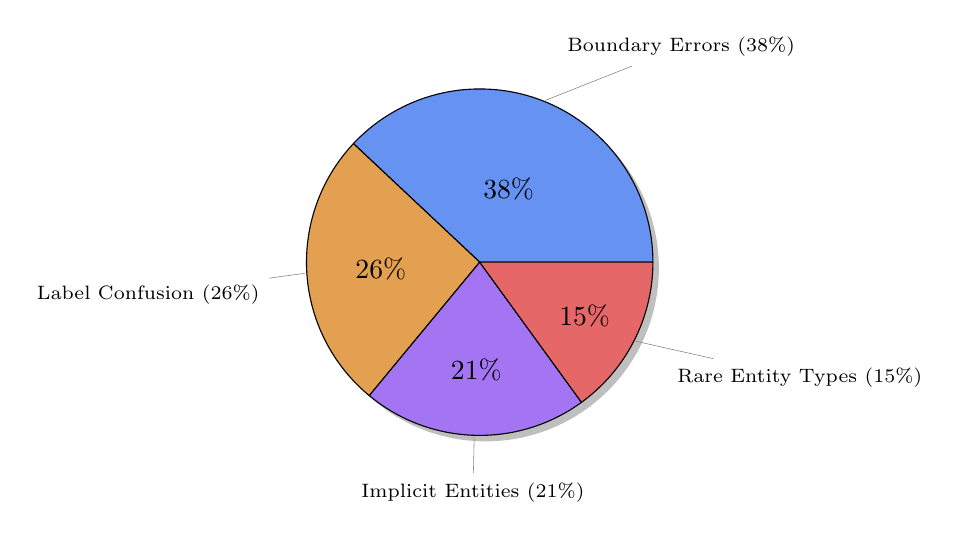
\begin{tikzpicture}
\pie[
  /tikz/every pin/.style={font=\scriptsize},
  text=pin,
  radius=2.2,
  color={colorA!70, colorD!70, colorE!70, colorC!70},
  style=drop shadow
]{
  38/Boundary Errors (38\%),
  26/Label Confusion (26\%),
  21/Implicit Entities (21\%),
  15/Rare Entity Types (15\%)
}
\end{tikzpicture}
\caption{Taxonomy of 127 error instances on the held-out test set.
Boundary errors (partial entity spans) represent the dominant failure mode;
implicit entity references present the most linguistically challenging class.}
\label{fig:error_taxonomy}
\end{figure}

\subsection{Comparison with Commercial Systems}

Table~\ref{tab:commercial} positions ClinicalMind against commercial and
research alternatives across eight capability dimensions. ClinicalMind is
the only system combining all eight capabilities: open-source access, audio
input, custom NER training, structured summarisation, FHIR output, entity
provenance, LLM distillation, and on-premises deployability.

\begin{table}[t]
\centering
\caption{Feature Comparison with Commercial and Research Systems}
\label{tab:commercial}
\setlength{\tabcolsep}{4pt}
\begin{tabular}{lcccc}
\toprule
\textbf{Feature} & \textbf{Ours} & \textbf{AWS} & \textbf{Nuance} & \textbf{NLP2FHIR} \\
\midrule
Open Source          & \checkmark & --      & --      & \checkmark \\
Audio Input          & \checkmark & \checkmark & \checkmark & -- \\
Custom NER Training  & \checkmark & --      & --      & Limited \\
Summarisation        & \checkmark & \checkmark & \checkmark & -- \\
FHIR Output          & \checkmark & Limited & --      & \checkmark \\
Entity Provenance    & \checkmark & \checkmark & Limited & \checkmark \\
LLM Distillation     & \checkmark & --      & --      & -- \\
On-Premises Deploy   & \checkmark & --      & --      & \checkmark \\
\bottomrule
\end{tabular}
\end{table}

%% ═════════════════════════════════════════════════════════════
\section{Discussion}
\label{sec:discussion}

\subsection{Clinical Applicability}

ClinicalMind's 12\,ms inference time enables entity extraction to run
concurrently with the clinical encounter, and FHIR-compatible output
facilitates EHR integration without custom interface development. The
open-source design enables institutional customisation and on-premises
deployment, eliminating the need to transmit sensitive patient audio or
text to external APIs—a critical differentiator for HIPAA-constrained
environments.

The extended entity schema fills a genuine clinical gap. Family history is
indispensable for genetic risk stratification in oncology and cardiology, yet
no existing English clinical dialogue NER system extracts it as a first-class
entity. CHRONIC\_DISEASE extraction enables automated construction of
longitudinal problem lists that differ meaningfully from acute encounter
diagnoses, supporting care coordination for complex patients.

\subsection{Knowledge Distillation as a Clinical NLP Strategy}

Our results validate knowledge distillation from LLMs to lightweight models
as a principled strategy for clinical NLP. The distilled model marginally
\emph{outperforms} its LLM teacher in overall F1, a finding we attribute to
the noise-reduction effect of the position-validation layer: the model is
trained on a \emph{curated subset} of Gemini's outputs rather than raw
predictions. This "curated distillation" paradigm may generalise beyond
clinical NER to other structured extraction tasks where training data quality
matters more than quantity.

The distillation approach offers five operational advantages over direct LLM
inference: (1)~\emph{Cost}: one-time annotation cost vs. per-inference charges;
(2)~\emph{Latency}: 12\,ms vs. 1.2\,s, enabling real-time use; (3)~\emph{Privacy}:
no patient data transmitted to external services; (4)~\emph{Reliability}: no
dependency on API availability or rate limits; (5)~\emph{Adaptability}: the
model can be fine-tuned on institution-specific data post-deployment.

\subsection{Limitations}

Several limitations bound the current evaluation. The dataset of 947 entities
across 7 types limits generalisation, particularly for rare categories
(AGE: $n\!=\!5$). Conversations may under-represent specialist clinical
settings (oncology, psychiatry, paediatrics). The evaluation is English-only;
clinical practice is inherently multilingual, and performance on accented
speech or code-switching conversations is unknown. Manual quality review
covered 50 conversations ($\sim$5\% of the corpus); a larger-scale inter-annotator
agreement study with multiple expert annotators is needed for rigorous validation.
ASR transcription errors propagate to NER: a joint end-to-end evaluation
including recognition errors would provide a more realistic performance bound.

\subsection{Ethical Considerations}

Clinical NLP systems carry patient safety implications. Boundary errors or
label confusions that reach downstream clinical decision support may affect
care quality. Demographic biases present in training dialogues may produce
systematically lower performance for patient subpopulations (elderly patients,
non-native English speakers, patients with speech disorders). We recommend
that all extracted entities be subject to clinician review before clinical
use, with ongoing monitoring for systematic errors across demographic groups.

In accordance with IEEE publication policies on AI-assisted research, we
disclose that Google Gemini was used to automate entity annotation for
training data generation. All Gemini-generated annotations were validated
algorithmically and reviewed by human experts; the final deployed model
operates entirely independently of any LLM.

%% ═════════════════════════════════════════════════════════════
\section{Conclusion}
\label{sec:conclusion}

We have presented ClinicalMind, a hybrid knowledge-distillation framework
for real-time medical conversation intelligence. Our principal findings are:

\begin{enumerate}
  \item Google Gemini produces high-quality clinical entity annotations
  (91.3\% entity-level accuracy) suitable for NER model training—the first
  published evaluation of Gemini for this task.
  \item A position-validation layer is \emph{essential}: without it,
  positional accuracy drops from 94.8\% to 67.2\%, causing F1 to degrade
  by 0.084 points in the distilled model.
  \item The distilled spaCy NER model achieves F1\,=\,0.872 at 12\,ms per
  conversation—100$\times$ faster than its LLM teacher at zero marginal
  cost—validating curated knowledge distillation as a practical clinical
  NLP strategy.
  \item Our seven-category schema, including Family History, Chronic Disease,
  and Vital Sign, fills an unmet gap in English clinical dialogue NER resources.
\end{enumerate}

Future work will expand the dataset across clinical specialties, introduce
multilingual capabilities, apply targeted data augmentation for rare entity
types, and conduct prospective evaluation with practising clinicians. We
release our annotation pipeline, entity schema, trained model, and experimental
code to support reproducible research in clinical conversation understanding.

%% ═════════════════════════════════════════════════════════════
\section*{Acknowledgment}

The authors disclose, in accordance with IEEE publication policies, that
Google Gemini (\texttt{gemini-2.5-flash}) was used to automate entity
annotation for the generation of NER training data. All LLM-generated
annotations were subsequently validated by Algorithm~\ref{alg:validation}
and reviewed by human domain experts. The final trained ClinicalMind model
operates entirely independently of any large language model.

%% ═════════════════════════════════════════════════════════════
\balance
\bibliographystyle{IEEEtran}
\begin{thebibliography}{29}

\bibitem{sinsky2016allocation}
C.~Sinsky, L.~Colligan, L.~Li, M.~Prgomet, S.~Reynolds, L.~Goeders,
J.~Westbrook, M.~Tutty, and G.~Blike,
``Allocation of physician time in ambulatory practice: A time and motion study
in 4 specialties,''
\emph{Ann.\ Intern.\ Med.}, vol.~165, no.~11, pp.~753--760, 2016.

\bibitem{shanafelt2022changes}
T.~D.~Shanafelt, C.~P.~West, C.~Sinsky, M.~Trockel, M.~Tutty, D.~V.~Satele,
L.~E.~Carlasare, and L.~N.~Dyrbye,
``Changes in burnout and satisfaction with work-life integration in physicians
and the general US working population between 2011 and 2020,''
\emph{Mayo Clin.\ Proc.}, vol.~97, no.~3, pp.~491--506, 2022.

\bibitem{johnson2016mimic}
A.~E.~W.~Johnson, T.~J.~Pollard, L.~Shen, L.~H.~Lehman, M.~Feng,
M.~Ghassemi, B.~Moody, P.~Szolovits, L.~A.~Celi, and R.~G.~Mark,
``MIMIC-III, a freely accessible critical care database,''
\emph{Sci.\ Data}, vol.~3, no.~1, pp.~1--9, 2016.

\bibitem{singhal2023large}
K.~Singhal, S.~Azizi, T.~Tu, S.~S.~Mahdavi, J.~Wei, H.~W.~Chung,
N.~Scales, A.~Tanwani, H.~Cole-Lewis, S.~Pfohl \emph{et al.},
``Large language models encode clinical knowledge,''
\emph{Nature}, vol.~620, no.~7972, pp.~172--180, 2023.

\bibitem{uzuner2011}
O.~Uzuner, B.~R.~South, S.~Shen, and S.~L.~DuVall,
``2010 i2b2/VA challenge on concepts, assertions, and relations in clinical
text,''
\emph{J.\ Am.\ Med.\ Inform.\ Assoc.}, vol.~18, no.~5, pp.~552--556, 2011.

\bibitem{lee2020biobert}
J.~Lee, W.~Yoon, S.~Kim, D.~Kim, S.~Kim, C.~H.~So, and J.~Kang,
``BioBERT: A pre-trained biomedical language representation model for
biomedical text mining,''
\emph{Bioinformatics}, vol.~36, no.~4, pp.~1234--1240, 2020.

\bibitem{alsentzer2019clinicalbert}
E.~Alsentzer, J.~R.~Murphy, W.~Boag, W.~H.~Weng, D.~Jin, T.~Naumann,
and M.~B.~A.~McDermott,
``Publicly available clinical BERT embeddings,''
in \emph{Proc.\ 2nd Clinical NLP Workshop}, 2019, pp.~72--78.

\bibitem{gu2021domain}
Y.~Gu, R.~Tinn, H.~Cheng, M.~Lucas, N.~Usuyama, X.~Liu, T.~Naumann,
J.~Gao, and H.~Poon,
``Domain-specific language model pretraining for biomedical NLP,''
\emph{ACM Trans.\ Comput.\ Healthcare}, vol.~3, no.~1, pp.~1--23, 2021.

\bibitem{kormilitzin2021med7}
A.~Kormilitzin, N.~Vaci, Q.~Liu, and A.~Nevado-Holgado,
``Med7: A transferable clinical NLP model for electronic health records,''
\emph{Artif.\ Intell.\ Med.}, vol.~118, p.~102086, 2021.

\bibitem{neumann2019scispacy}
M.~Neumann, D.~King, I.~Beltagy, and W.~Ammar,
``ScispaCy: Fast and robust models for biomedical NLP,''
in \emph{Proc.\ 18th BioNLP Workshop}, 2019, pp.~319--327.

\bibitem{henry2020n2c2}
S.~Henry, K.~Buchan, M.~Filannino, A.~Stubbs, and O.~Uzuner,
``2018 n2c2 shared task on adverse drug events and medication extraction,''
\emph{J.\ Am.\ Med.\ Inform.\ Assoc.}, vol.~27, no.~1, pp.~3--12, 2020.

\bibitem{tan2024llm}
B.~Tan, Z.~Yang, A.~Gokhan, Z.~Chen, D.~Roth, and K.~McKeown,
``Large language models for data annotation and synthesis: A survey,''
in \emph{Proc.\ EMNLP}, 2024.

\bibitem{he2024crowdsource}
S.~He, H.~Fang, P.~Mozannar, P.~Kamar, and M.~Bansal,
``If in a crowdsourced data annotation pipeline, a GPT-4,''
in \emph{Proc.\ CHI}, 2024, pp.~1--22.

\bibitem{hu2024improving}
Y.~Hu, I.~J.~Kelley, O.~Patterson, G.~Divita, S.~Luther, and R.~Tao,
``Improving large language models for clinical named entity recognition via
prompt engineering,''
\emph{J.\ Am.\ Med.\ Inform.\ Assoc.}, vol.~31, no.~9, pp.~1812--1820, 2024.

\bibitem{li2023lapras}
Y.~Li, S.~Krishnamoorth, S.~Chen, and W.~Wang,
``Lapras: Language model for labeling with rationalization and
self-consistency,''
\emph{arXiv preprint arXiv:2305.12106}, 2023.

\bibitem{abacha2023mtsdialog}
A.~B.~Abacha, W.~Yim, Y.~Fan, and T.~Lin,
``An empirical study of clinical note generation from doctor-patient
encounters,''
in \emph{Proc.\ EACL}, 2023, pp.~2291--2302.

\bibitem{chen2022imcs21}
W.~Chen, Z.~Li, H.~Fang, Q.~Yao, C.~Zhong, J.~Hao, Q.~Zhang, X.~Huang,
J.~Peng, and W.~Heng,
``A benchmark for automatic medical consultation system,''
\emph{Bioinformatics}, vol.~39, no.~1, p.~btac817, 2022.

\bibitem{wang2024notechat}
K.~Wang, J.~Giorgi, R.~Bhaskar, C.~Wang, and B.~C.~Wallace,
``NoteChat: A dataset of synthetic patient-physician conversations conditioned
on clinical notes,''
in \emph{Findings ACL}, 2024.

\bibitem{hodgson2016evaluating}
T.~Hodgson, B.~R.~Magrabi, and F.~Coiera,
``Evaluating the efficiency of speech recognition in medical transcription,''
\emph{Int.\ J.\ Med.\ Inform.}, vol.~113, pp.~25--30, 2016.

\bibitem{chiu2021speech}
C.~Chiu, J.~Tripathi, K.~Chou, C.~Co, N.~Jaitly, D.~Jaunzeikare,
A.~Kannan, P.~Nguyen, H.~Sak, and A.~Sankar,
``Speech recognition for medical conversations,''
in \emph{Proc.\ Interspeech}, 2021, pp.~2972--2976.

\bibitem{radford2023robust}
A.~Radford, J.~W.~Kim, T.~Xu, G.~Brockman, C.~McLeavey, and I.~Sutskever,
``Robust speech recognition via large-scale weak supervision,''
in \emph{Proc.\ ICML}, 2023, pp.~28492--28518.

\bibitem{koenecke2024}
A.~Koenecke, A.~Nam, E.~Lake, J.~Nudell, M.~Quartey, Z.~Mengesha,
C.~Tober, D.~Littman, and D.~Jurafsky,
``Careless whisper: Speech-to-text hallucination harms,''
in \emph{Proc.\ ACM FAccT}, 2024.

\bibitem{zhang2024whispermed}
J.~Zhang, Y.~Zhou, and L.~Chen,
``Whisper-Med: Towards medical domain-adapted ASR,''
\emph{arXiv preprint arXiv:2402.10973}, 2024.

\bibitem{kocaman2021sparknlp}
V.~Kocaman and D.~Talby,
``Spark NLP: Natural language understanding at scale,''
\emph{Software Impacts}, vol.~8, p.~100058, 2021.

\bibitem{aws2023healthscribe}
Amazon Web Services,
``AWS HealthScribe,'' 2023. [Online]. Available:
\url{https://aws.amazon.com/healthscribe/}

\bibitem{tierney2024ambient}
A.~A.~Tierney, G.~Gayre, B.~Hoberman, B.~Mattern, M.~Ballesca, P.~Kipps,
N.~Bharath, C.~Siegel, and J.~Pfeffer,
``Ambient AI scribes to alleviate the burden of clinical documentation,''
\emph{NEJM Catalyst}, vol.~5, no.~3, 2024.

\bibitem{hong2019nlp2fhir}
N.~Hong, A.~Wen, F.~Shen, S.~Sohn, C.~Wang, H.~Liu, and G.~Jiang,
``Developing a scalable FHIR-based clinical data normalization pipeline,''
\emph{JAMIA Open}, vol.~2, no.~4, pp.~570--579, 2019.

\bibitem{chen2024fhirgpt}
S.~Chen, M.~Peng, C.~Wen, and J.~Zhu,
``FHIR-GPT: Enhancing health interoperability with large language models,''
in \emph{Proc.\ AMIA Annual Symposium}, 2024.

\bibitem{vanveen2024adapted}
D.~Van~Veen, C.~Van~Uden, L.~Berry, Y.~Chen, and A.~Rajpurkar,
``Adapted large language models can outperform medical experts in clinical
text summarization,''
\emph{Nature Med.}, vol.~30, no.~4, pp.~1134--1142, 2024.

\end{thebibliography}

\end{document}
